\label{chuong_3}

Trong các hệ thống học máy tại biên (TinyML), tập dữ liệu huấn luyện chất lượng cao là yếu tố nền tảng để mô hình hoạt động tốt trên thực tế. Do bài toán phát hiện bất thường gặp vấn đề khan hiếm dữ liệu lỗi, đề tài tiếp cận theo hướng học không giám sát, yêu cầu một tập dữ liệu nền (Background Dataset) chuẩn xác phản ánh các trạng thái vận hành bình thường của thiết bị. Chương này trình bày quy trình xây dựng tập dữ liệu thực tế, các kỹ thuật tăng cường dữ liệu và quá trình huấn luyện mô hình tự mã hóa ba trạng thái.

\section{Quá trình thu thập dữ liệu thực tế}

Để xây dựng tập dữ liệu phản ánh đặc tính vật lý của máy giặt, một trạm thu thập dữ liệu chuyên dụng dựa trên vi điều khiển Seeed Studio XIAO ESP32-S3 đã được thiết kế và gắn trực tiếp lên lồng giặt để đo đạc thực địa.

\subsection{Xây dựng giao thức truyền nhận dữ liệu tốc độ cao định dạng nhị phân}

Thu thập dữ liệu đa cảm biến (âm thanh 8 kHz + gia tốc 1 kHz) qua cổng Serial bằng văn bản ASCII sẽ gây độ trễ phân giải cao, dẫn đến tràn bộ đệm và mất mẫu. Để khắc phục, đồ án triển khai giao thức truyền dẫn nhị phân (Binary Protocol) tùy chỉnh qua UART ở tốc độ baud 921600. ESP32 trích xuất vector đặc trưng 19 chiều tại thiết bị biên, sau đó đóng gói vào một cấu trúc chuẩn:

\begin{itemize}
    \item \textbf{Cấu trúc Payload:} Mỗi gói tin bắt đầu bằng hai byte đồng bộ (Sync word) \texttt{0xAA 0xBB}, tiếp theo là 19 giá trị float (76 bytes), và kết thúc bằng một byte kiểm tra lỗi (Checksum).
    \item \textbf{Hiệu năng:} Truyền trực tiếp khối nhớ nhị phân thay vì chuyển đổi sang chuỗi tiết kiệm khoảng 60\% băng thông kênh truyền, đảm bảo thu thập liên tục mà không quá tải phần cứng.
\end{itemize}

\subsection{Tự động hóa quy trình thu thập và kiểm soát chất lượng dữ liệu}

Một kịch bản Python (\texttt{dataCollection.py}) được phát triển để tự động hóa quy trình thu thập cho các chu kỳ kéo dài 45 - 90 phút.

\begin{itemize}
    \item \textbf{Tự động hóa phân mảnh (Windowing):} Kịch bản liên tục đọc luồng Serial, căn lề theo byte đồng bộ để giải mã mảng nhị phân. Mỗi tệp ghi 5 giây được tách thành 5 cửa sổ 1 giây, tương ứng 5 mẫu đặc trưng độc lập, rồi lưu trữ dưới định dạng ma trận NumPy (\texttt{.npy}).
    \item \textbf{Kiểm soát chất lượng (Data Quality Control):} Quá trình thu nhận thực hiện hai bước kiểm tra:
    \begin{enumerate}
        \item \textit{Xử lý nhiễu:} Tự động loại bỏ các mẫu chứa giá trị \texttt{NaN} hoặc \texttt{Inf} (do xung đột bus I2C hoặc nhiễu điện từ).
        \item \textit{Đồng bộ hóa dải năng lượng:} Áp dụng kỹ thuật \textit{Audio Volume Shifting}, giới hạn năng lượng phổ Mel trong dải chuẩn $[-80, 0]$ dB. Thao tác này giúp khắc phục sai lệch biểu diễn dữ liệu giữa môi trường huấn luyện (Python) và môi trường thực thi (C++).
    \end{enumerate}
\end{itemize}

\subsection{Thống kê phân phối và xử lý sự mất cân bằng dữ liệu (Data Imbalance)}
\label{subsec:data_distribution_balance}

Sau nhiều phiên đo đạc các chu trình giặt thực tế, hệ thống có tập dữ liệu gốc (Raw Dataset) gồm 14.000 mẫu (khoảng 20 giờ vận hành). Dữ liệu được phân nhóm tự động thành ba cụm trạng thái dựa trên phương sai trục Z (Hình~\ref{fig:varZ_tristate}), phản ánh mất cân bằng tự nhiên của chu trình giặt:

\begin{itemize}
    \item \textbf{Tập GENTLE (Pha giặt/ngâm):} 12.853 mẫu (khoảng 91,8\%). Tỷ trọng lớn phù hợp vì đây là pha chiếm thời gian dài nhất.
    \item \textbf{Tập STRONG (Pha xả/đảo lồng):} 551 mẫu (3,9\%). Pha này diễn ra trong thời gian ngắn khi máy đảo lồng để xả nước.
    \item \textbf{Tập SPIN (Pha vắt):} 596 mẫu (4,3\%). Pha vắt tốc độ cao kéo dài vài phút ở cuối chu trình.
\end{itemize}

\begin{figure}[H]
    \centering
    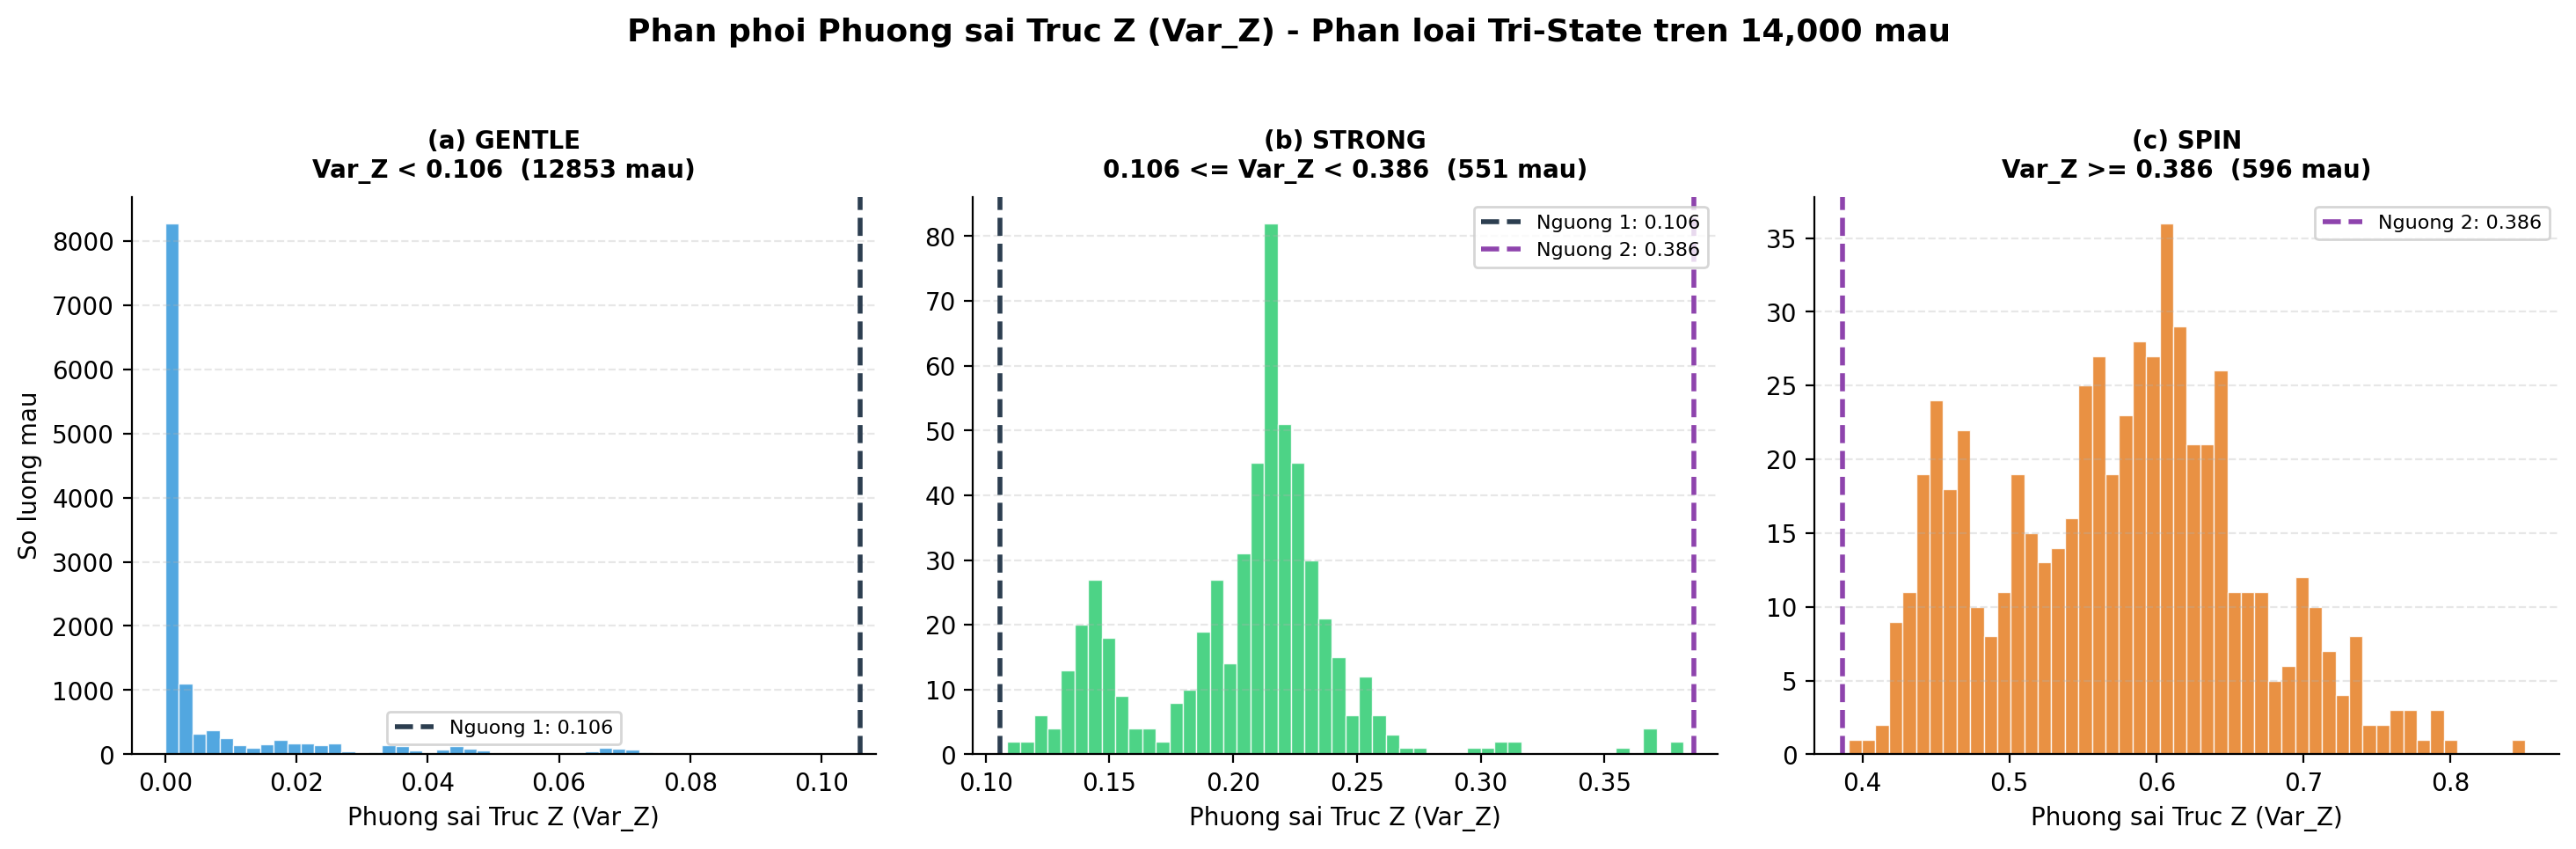
\includegraphics[width=0.95\linewidth]{chap3/image/fig_varZ_tristate.png}
    \caption[Phân phối phương sai trục Z]{Phân phối thực nghiệm của phương sai trục Z ($Var\_Z$) trên tập dữ liệu 14.000 mẫu. Hai ngưỡng phân hoạch tại 0.106 và 0.386 tạo ra ba vùng phân bố tách biệt rõ rệt.}
    \label{fig:varZ_tristate}
\end{figure}

Các ngưỡng phân hoạch trạng thái được xác định tự động thông qua thuật toán \textbf{K-Means Clustering}. Thuật toán gom cụm phương sai trục Z thành 3 nhóm, từ đó tính toán các ranh giới $\tau_1$ và $\tau_2$ tại điểm trung vị giữa hai cụm kế cận. Cách tiếp cận này cho phép hệ thống thích nghi với mức rung động khác nhau của từng loại lồng giặt.

Tuy nhiên, chênh lệch phân phối ở tỷ lệ 92:4:4 tạo vấn đề cho huấn luyện. Nếu dùng trực tiếp tập dữ liệu thô, mạng nơ-ron tự mã hóa sẽ thiên lệch về phía tập GENTLE, giảm độ chính xác tái tạo ở các pha STRONG và SPIN. Để khắc phục, thay vì giảm lấy mẫu (Undersampling), đồ án áp dụng chiến lược tăng cường dữ liệu (Data Augmentation) \cite{ref_1_8}. Ba kỹ thuật được kết hợp:

\begin{enumerate}
    \item \textbf{Magnitude Scaling:} Nhân biên độ rung với hệ số ngẫu nhiên trong khoảng $[0.8, 1.2]$ để giả lập sự thay đổi tải trọng đồ giặt.
    \item \textbf{Audio Volume Shifting:} Tịnh tiến năng lượng phổ Mel ngẫu nhiên từ $-5$ dB đến $+2$ dB nhằm giả lập sai số về khoảng cách thu âm.
    \item \textbf{Per-axis Jittering:} Thêm nhiễu Gauss độc lập vào từng trục gia tốc để tăng khả năng chống rung động vi mô.
\end{enumerate}

Sau khi tăng cường dữ liệu, các tập GENTLE, STRONG và SPIN lần lượt có 20.000, 10.000 và 10.000 mẫu, với tỷ lệ cân bằng hơn là 2:1:1 (Hình~\ref{fig:data_distribution}).

\begin{figure}[H]
    \centering
    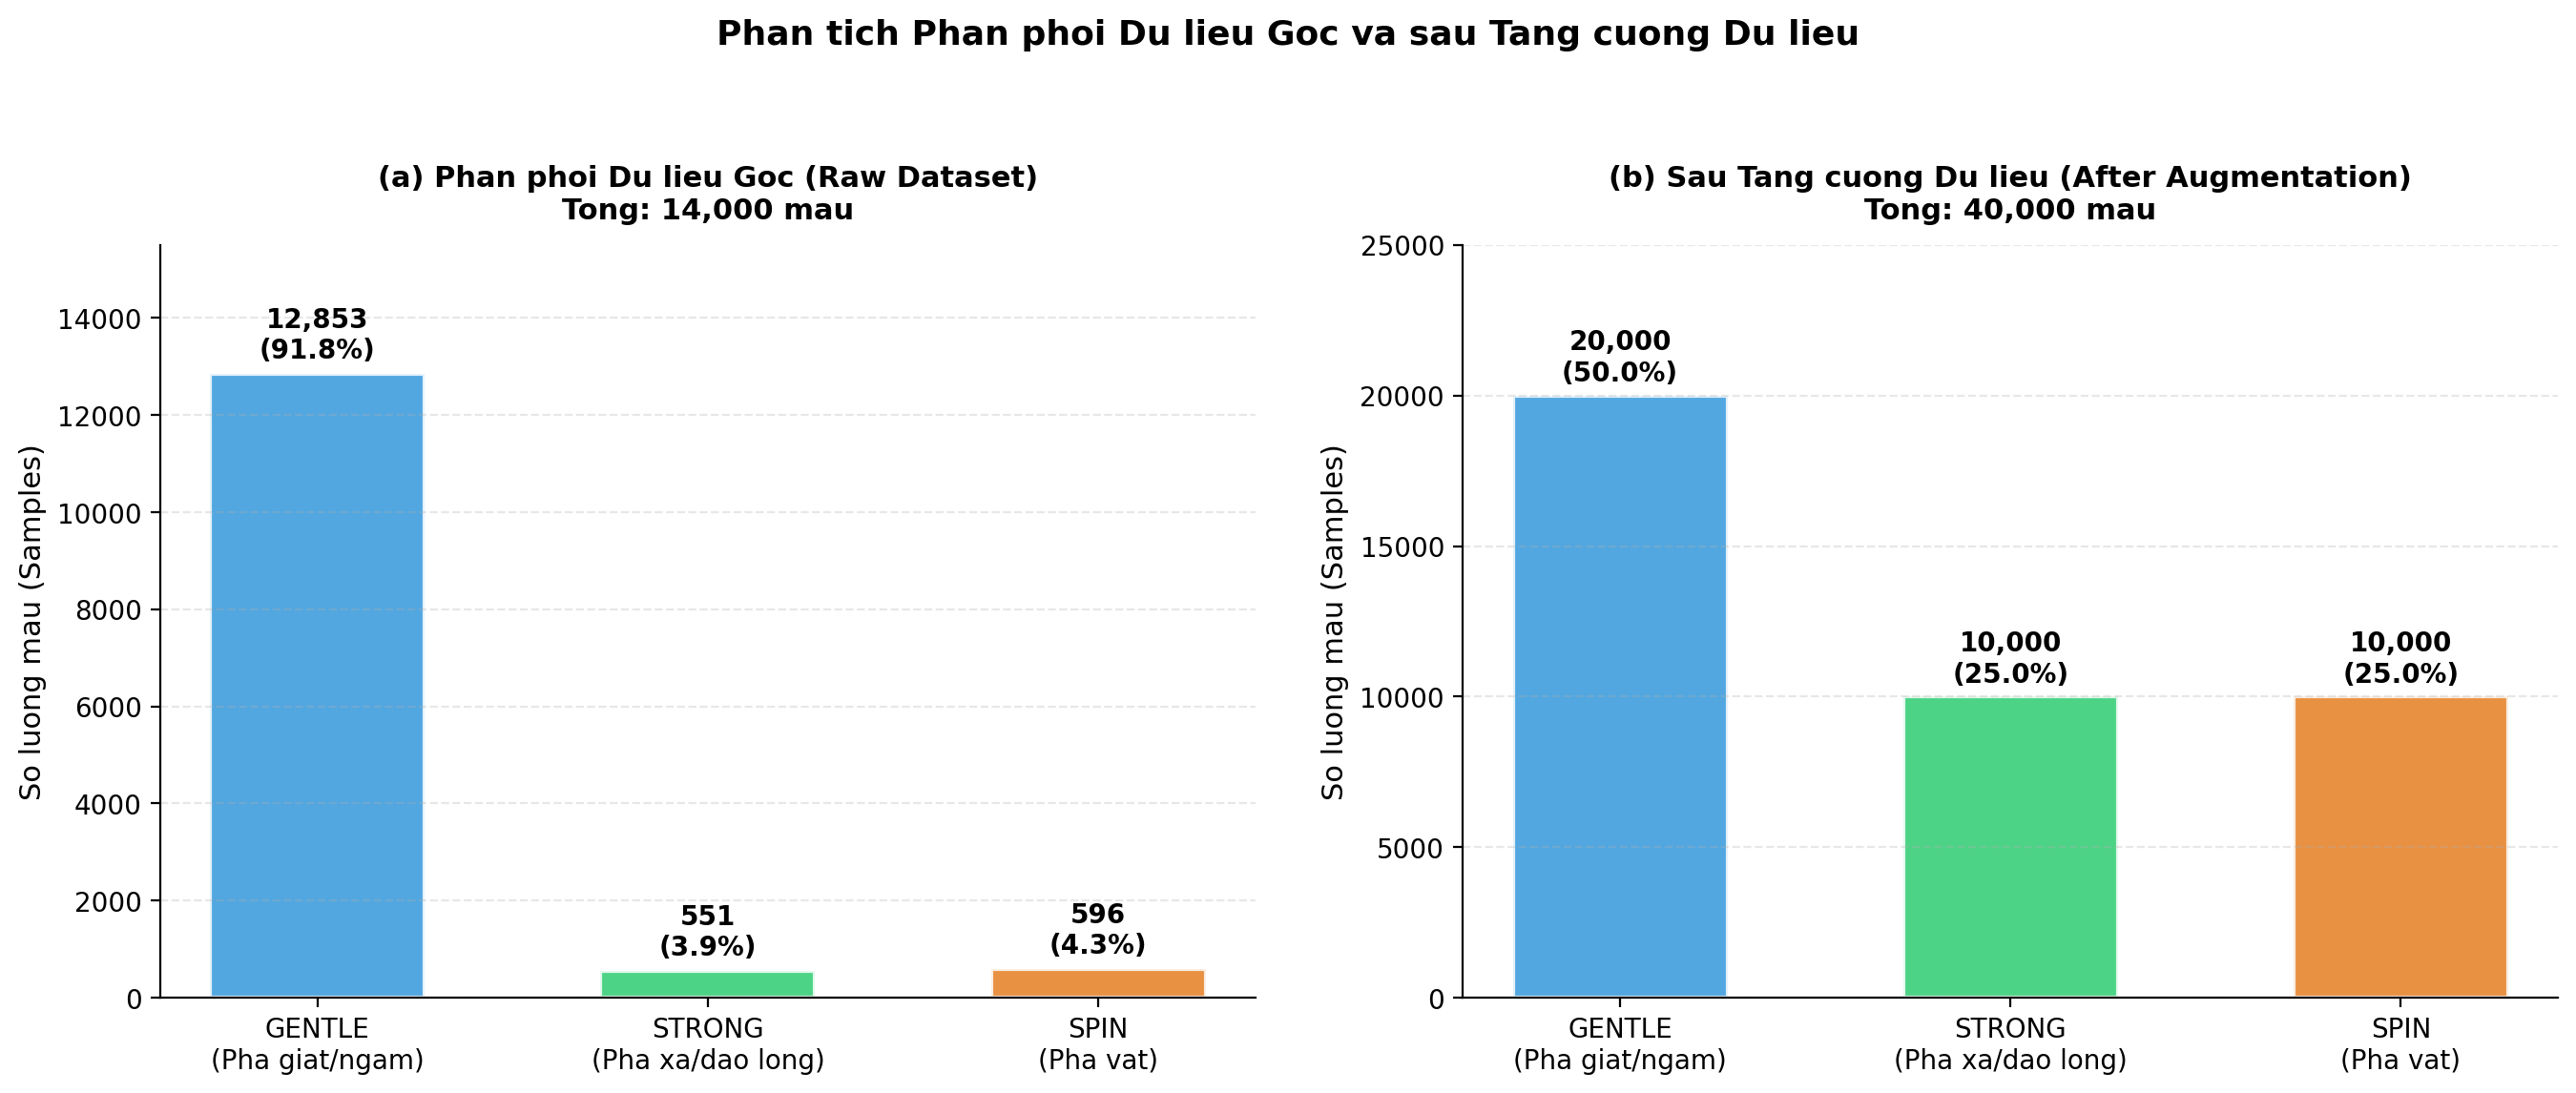
\includegraphics[width=1.0\linewidth]{chap3/image/fig_data_distribution.png}
    \caption[Phân phối dữ liệu trước và sau tăng cường]{Phân phối dữ liệu ba trạng thái trước và sau quá trình tăng cường. Tỷ lệ chênh lệch ban đầu (92:4:4) được cân bằng về mức 2:1:1.}
    \label{fig:data_distribution}
\end{figure}

% ==============================================================================
% DANH MỤC TÀI LIỆU THAM KHẢO TRÍCH DẪN (MỤC 3.1)
% ==============================================================================
% \bibitem{ref_1_8} M. Abdallah et al., "Anomaly Detection and Inter-Sensor Transfer Learning on Smart Manufacturing Datasets," Sensors, vol. 23, no. 1, p. 486, 2023.
